\chapter{Related Work}\label{chap:related-work}
As this thesis brings together Predictive Process Monitoring with an approach from the area of sequence prediction, this chapter on related literature presents selected publications from both domains. To highlight the multitude of approaches and aforementioned obstacles to comparability, used technologies and datasets are quoted wherever possible.

Publications related to Predictive Process Monitoring are presented in \autoref{sec:related-work-predictive-process-monitoring}, with the chapter ending in a detailed presentation of the works of Evermann et al.~\cite{evermann2016} and Schönig et al.~\cite{schoenig2018} Similarly, \autoref{sec:related-work-sequence-prediction} presents other sequence prediction approaches from NLP and ends with in-depth information on the publication from Shibata et al.~\cite{shibata2016bipartite} we took as an inspiration.

\section{Predictive Process Monitoring}
\label{sec:related-work-predictive-process-monitoring}
Hauder et al. mention numerous research challenges in the domain of ACM, among them an active support system for knowledge workers \cite{hauder2014}.
The need for such a system is emphasized by Francescomarino et al. in an extensive literature review, where it has been found that few prediction approaches target the next activity \cite{francescomarino2018}.\\

\marginpar{CoCaMa is an abbreviation for a project called Collaborative Case Management that appears to be retired: \href{http://archive.li/uZFnN}{archive.li/uZFnN}}
An example for how a support system \cite{hauder2014} for case workers might look like, is given by Huber, who has developed a next-step prediction and recommendation system~\cite{huber2015}. The system is prototypically implemented within CoCaMa, a case management application.

The predictions made as follows: After gathering the training data from various sources via an extract, transform and load (ETL) process, several \textit{Next Models} are constructed. The Next Models are a collection of predictive models used to predict the next activity, focused on different criteria: remaining time, constraint violation, decisions based on case-specific data, and case outcome. The weighting of the predictions from these individual models is non-trivial and extensively discussed. Huber uses decision trees from the WEKA \cite{web:weka} machine learning toolkit to implement them. The system has been evaluated with 25 hand-made case logs \cite{huber2015}.\\

Polato et al. make use of data attributes attached to events in their work for improving the prediction of the remaining time of business process instances \cite{polato2014}. During feature engineering, their training data is enriched with information about possible other activities. With support vector regression from the WEKA toolkit~\cite{web:weka} and default parameters, they are able to reach $6\%$ and $9\%$ MAPE on two non-public data-sets of 5000 and 1500 traces.\\

Metzger et al. predict constraint violation of a case by comparing fundamentally different prediction models and combining them into an ensemble. The ensemble is tested with different voting mechanisms, e.g. majority voting or recall-orientation. They argue that late and precise or early and incorrect predictions are equally worthless for interventions, leading them to establish that between $60\% - 85\%$ progress into the process, predictions become stable and precise.

Three approaches are used to predict constraint violations: constraint satisfaction, Quality-of-Service (QoS) violation checks and machine learning. The two former models use rules to predict a process outcome while the latter is a trained neural network. For it, Metzger et. al use the ANN implementation from the WEKA machine learning toolkit with a single hidden layer. 

The authors are able to formulate rules for the two other models because the process at hand is very rigid and well defined: The Cargo 2000 process is a standard proposed by the International Air Transport Association (IATA) \cite{metzger2015}. Their non-public dataset of 3942 traces and 56082 events was used $\frac{2}{3}$ for training the remainder for testing.\\

Also aiming at predicate fulfilment were Francescomarino et al. when they they organized predictive models in a clustered fashion \cite{francescomarino2015}. Having clustered the training data, one model was trained on each cluster. Then, to obtain a prediction, the cluster for a new data item needs to found, and the corresponding model selected. Furthermore, the authors varied the probability threshold for accepting a prediction and measured how it affected the point in process progress at which the predictions become stable (similar to Metzger et al.). They referred to this characteristic as \textit{earliness}. Their approach, implemented as a ProM plugin called \textit{Predictive Process Monitoring}, uses two different clustering methods (k-means, DBSCAN) and two different types of predictive models (decision trees and random forests). It was tested on the BPIC2011~\cite{BPIC2011} dataset.

Picking up on Francescomarinos approach and training a neural network for every cluster was heavily considered at the beginning of this thesis but foregone because of the possibility to use embedding layers which allow the ANN to cluster itself.\\

Approaching the process prediction in a different fashion are Böhmer et al. with a method rooted in heuristic analysis \cite{boehmer2018probability}. Based on the fact that the black-box nature of ANNs makes their predictions and inner workings very hard to comprehend, they argue that the amount of trust that users put into their predictions results is limited. As potentially large organizational changes could be made due to the predictions, the authors perceive it of importance to explain alternative futures which were not classified as being most probable and explain the aspects which motivated specific prediction results.
Böhmer et al. approximate trace similarities with the Damerau-Levenstein method and a custom cost function. Using this method, they filter historic traces to produce a set of similar executions. From this set, probability distributions are mined, with the most probable behaviour ultimately used as the final prediction \cite{boehmer2018probability}.\\

Klinkmüller et al. enrich their training dataset with markers that encode subsequence occurrence \cite{klinkmuller2018reliablemonitoring}. Doing so on a synthetic dataset, they are able to increase the accuracy of a random forest in comparison to a baseline that is not using the engineered subsequence features. This approach is similar to that of Shibata et al. \cite{shibata2016bipartite}, which is thoroughly examined in the next section. Furthermore, the authors find that training classifiers on complete traces is preferable to trace truncation.\\

Building upon each other are the works by Evermann et al. \cite{evermann2016} and Schönig et al. \cite{schoenig2018}.

Evermann et al. remark the lack of research on next event predictions and have successfully demonstrated the applicability of LSTM neural networks in the context of predicting the next activity. Using a neural network implemented with Tensorflow, precisions between $60\%$ to $90\%$ on the BPIC2012 and BPIC2013 datasets are achieved. Evermann et al. want their work to be understood as a "demonstration of the applicability of the approach and the potential for future work". The authors highlight that their work lacks use of data attributes during model training. 

Schönig et al. \cite{schoenig2018} picked up on the last point and demonstrated on BPIC datasets from 2017 that using data attributes complementary to the event names does increase prediction accuracy. Schönig et al. implemented their solution with Keras and trained it with stratified 5-fold cross-validation.
The data was preprocessed with one-hot encoding for categorical variables and min-max-normalization for continuous features. Also, the work nicely demonstrates that an increasing number of included data attributes can improve accuracy \cite[p.5]{schoenig2018}, without referring to any of their statistical properties. Their approach reaches accuracies around $90\%$, depending on its configuration.

\begin{figure}
\centering
\subfloat[][Architecture used by Evermann et al. \cite{evermann2016}.]{
    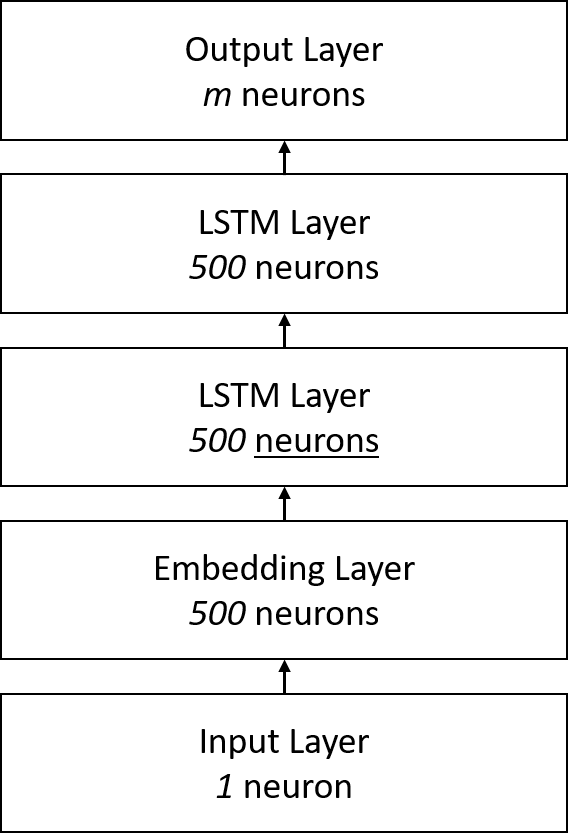
\includegraphics[width=0.3\textwidth]{gfx/evermann-network-architecture.png}
    \label{fig:evermann-architecture}
}
\qquad
\subfloat[][Architecture used by Schönig et al. \cite{schoenig2018}.]{
    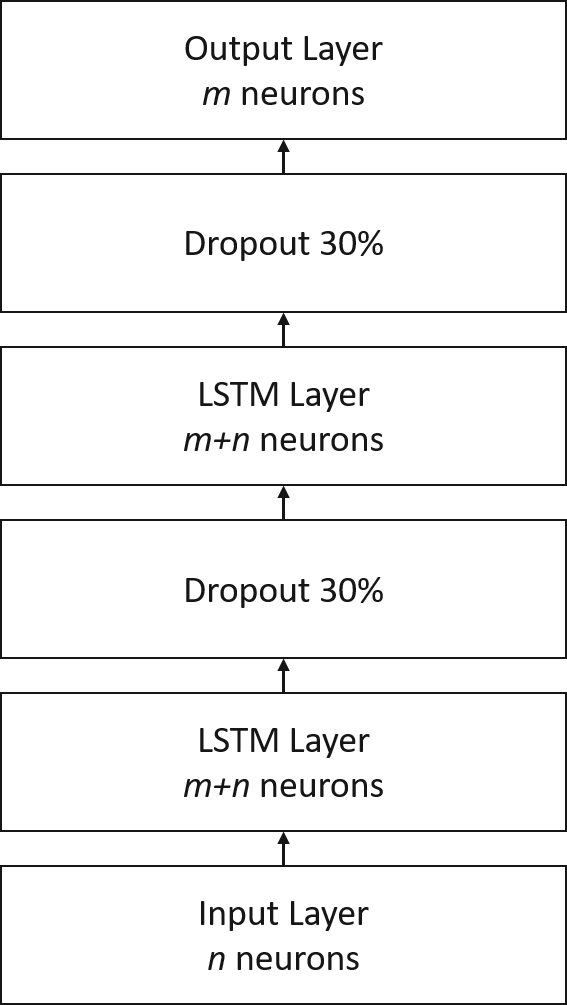
\includegraphics[width=0.3\textwidth]{gfx/schoenig-network-architecture.png}
    \label{fig:schoenig-architecture}
}
\caption{An overview of the reverse-engineered networks that are used as a comparison in this thesis.}
\label{fig:benchmark-architectures}
\end{figure}

The works of Evermann et al. and Schönig et al. are important for benchmarking our approach, as they both used BPIC data and the source code for both works has been made available. In close collaboration with the two authors, their neural networks were reverse-engineered and also the architectures in \autoref{fig:benchmark-architectures} were confirmed to be correct.

Clearly, Evermann's architecture left an inspiring impression with Schönig, who decided to remove the Embedding layer and adapt unit counts and activation functions. In our conversation, Schönig argued that the Embedding was not needed, as the number of unique events was a lot lower than that of words in a text, for which Embeddings were originally developed. Where Evermann et al. used stochastic gradient descent (SGD) with a manual adaption of learning rate decay to $75\%$ after the 25th epoch, Schönig et al. use RMSprop with default values to optimize the network's loss. Furthermore, Schönig et al. fed the training data into their networks in a windowed fashion, contrary to Klinkmüller's suggestion that this might reduce accuracy~\cite{klinkmuller2018reliablemonitoring}. Furthermore, both Evermann and Schönig have not made their predictions case-specific, but chose to predict the next event in the complete stream.
\todo[inline]{This is a pretty big difference, maybe stress more?}

\section{Sequence prediction}
\label{sec:related-work-sequence-prediction}
Colocated with the International Conference in Grammatical Inference 2016 (ICGI) was a competition called SPiCE\ "about guessing the next element in a sequence" \cite{web:spice}. The competition consisted of twelve different datasets to use for predicting the next word. Most entries submitted to this competition made use of RNNs with LSTM cells to do so.\\

\begin{figure}
    \centering
    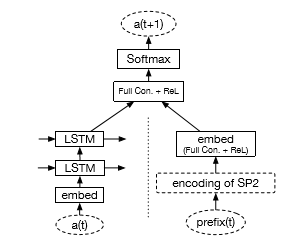
\includegraphics[height=.4\textwidth]{gfx/spice-winner-architecture.png}
    \caption{The neural network architecture of the winning submission at the SPiCE competition by Shibata et al. \cite{shibata2016bipartite}.}
    \label{fig:spice-winner-architecture}
\end{figure}

The winning submission by Shibata et al. uses a bipartite network architecture training separate layers on different features of the same sentence. The results of these separate layers are then merged in the middle hidden layers to produce a single output \cite{shibata2016bipartite}, as \autoref{fig:spice-winner-architecture} shows. Architectural similarities with Schönig et al. and Evermann et al. are especially prominent in the left part of Shibata's model.
While one half of the layers are trained on the most recent word of the sentence, the other half is trained on the prefix of that word. As this prefix can be of any length, Shibata et al. propose a binary bag-of-words encoding, representing the states of a SP-2 automaton.

SP-$k$ languages are used to describe certain long-term dependencies through forbidden subsequences. For example, if $\langle a,b \rangle$ is forbidden, then no $b$ may ever occur after $a$. As per Heinz, who assisted Shibata, deterministic finite automatons (DFA) can also be used to characterize SP-$k$ languages, if its states encode the subsequences of size $k-1$  present in the previous prefixes \cite{heinz2010estimatingSP}. To make this concept more tangible, \autoref{tab:sp2-encoding} illustrates a small example. The authors argue that LSTMs are not completely understood and it has not been proven that they are fully capable of recognizing sequences themselves, which is why these features should assist the network. To prove their point, they compare the SP-$k$ bipartite architecture with a basic one that is nearly identical to the one by Evermann et al in \autoref{fig:evermann-architecture}. The performance differences between the two models are acknowledged as generally "slight", while the basic architecture performs "significantly worse on three problems". 

\begin{table}
    \centering
    \begin{tabular}{cclccccc}
        \hline
          &      &              & \multicolumn{5}{c}{SP-2 vector}\\
        t & a(t) & prefix(a(t)) & [a & b & c & d & e]\\
        \hline
        0 & a    & a            & [1 & 0 & 0 & 0 & 0]\\
        1 & d    & ad           & [1 & 0 & 0 & 1 & 0]\\
        2 & a    & ada          & [1 & 0 & 0 & 1 & 0]\\
        3 & c    & adac         & [1 & 0 & 1 & 1 & 0]\\
        4 & d    & adacd        & [1 & 0 & 1 & 1 & 0]\\
        \hline
    \end{tabular}
    \caption{Prefixes encoded with SP-2. As $t$ progresses, more and more single-item subsequences ($k-1=1$) are marked as occurred. The alphabet is $I=\{a,b,c,d,e\}$. This example is taken from Shibata et al.  \cite{shibata2016bipartite}.}
    \label{tab:sp2-encoding}
\end{table}

Attention, a fairly new development in the domain of ANNs, has been leveraged by Kokkinos et al. in a tree-structured neural network to classify sentiments in sentences \cite{kokkinos2017structural}. In a detailed comparison with other works, their bipartite tree approach yields the highest accuracy on the Stanford Sentiment Treebank dataset. While the proposition of tree-structured Gated Recurrent Units (GRUs, a variant of LSTM units) and their use of attention is arguably the main contribution of this work, they make use of a bipartite network architecture and word embeddings as well. This gives further appeal to the idea.